%%%%%%%%%%%%%%%%%%%%%%%%%%%%%%%%%%%%%%%
% Wenneker Resume/CV
% LaTeX Template
% Version 1.1 (19/6/2016)
%
% This template has been downloaded from:
% http://www.LaTeXTemplates.com
%
% Original author:
% Frits Wenneker (http://www.howtotex.com) with extensive modifications by 
% Vel (vel@LaTeXTemplates.com)
%
% License:
% CC BY-NC-SA 3.0 (http://creativecommons.org/licenses/by-nc-sa/3.0/
%
%%%%%%%%%%%%%%%%%%%%%%%%%%%%%%%%%%%%%%

%----------------------------------------------------------------------------------------
%	PACKAGES AND OTHER DOCUMENT CONFIGURATIONS
%----------------------------------------------------------------------------------------

\documentclass[a4paper,12pt]{memoir} % Font and paper size

%%%%%%%%%%%%%%%%%%%%%%%%%%%%%%%%%%%%%%%%%
% Wenneker Resume/CV
% Structure Specification File
% Version 1.1 (19/6/2016)
%
% This file has been downloaded from:
% http://www.LaTeXTemplates.com
%
% Original author:
% Frits Wenneker (http://www.howtotex.com) with extensive modifications by 
% Vel (vel@latextemplates.com)
%
% License:
% CC BY-NC-SA 3.0 (http://creativecommons.org/licenses/by-nc-sa/3.0/)
%
%%%%%%%%%%%%%%%%%%%%%%%%%%%%%%%%%%%%%%%%%

%----------------------------------------------------------------------------------------
%	PACKAGES AND OTHER DOCUMENT CONFIGURATIONS
%----------------------------------------------------------------------------------------

\usepackage{XCharter} % Use the Bitstream Charter font
\usepackage[utf8]{inputenc} % Required for inputting international characters
\usepackage[T1]{fontenc} % Output font encoding for international characters

\usepackage[top=1cm,left=1cm,right=1cm,bottom=1cm]{geometry} % Modify margins

\usepackage{graphicx} % Required for figures

\usepackage{flowfram} % Required for the multi-column layout

\usepackage{url} % URLs

\usepackage[usenames,dvipsnames]{xcolor} % Required for custom colours

\usepackage{tikz} % Required for the horizontal rule

\usepackage{enumitem} % Required for modifying lists
\setlist{noitemsep,nolistsep} % Remove spacing within and around lists

\setlength{\columnsep}{\baselineskip} % Set the spacing between columns

% Define the left frame (sidebar)
\newflowframe{0.2\textwidth}{\textheight}{0pt}{0pt}[left]
\newlength{\LeftMainSep}
\setlength{\LeftMainSep}{0.2\textwidth}
\addtolength{\LeftMainSep}{1\columnsep}
 
% Small static frame for the vertical line
\newstaticframe{1.5pt}{\textheight}{\LeftMainSep}{0pt}
 
% Content of the static frame with the vertical line
\begin{staticcontents}{1}
\hfill
\tikz{\draw[loosely dotted,color=RoyalBlue,line width=1.5pt,yshift=0](0,0) -- (0,\textheight);}
\hfill\mbox{}
\end{staticcontents}
 
% Define the right frame (main body)
\addtolength{\LeftMainSep}{1.5pt}
\addtolength{\LeftMainSep}{1\columnsep}
\newflowframe{0.7\textwidth}{\textheight}{\LeftMainSep}{0pt}[main01]

\pagestyle{empty} % Disable all page numbering

\setlength{\parindent}{0pt} % Stop paragraph indentation

%----------------------------------------------------------------------------------------
%	NEW COMMANDS
%----------------------------------------------------------------------------------------

\newcommand{\userinformation}[1]{\renewcommand{\userinformation}{#1}} % Define a new command for the CV user's information that goes into the left column

\newcommand{\cvheading}[1]{{\Huge\bfseries\color{RoyalBlue} #1} \par\vspace{.6\baselineskip}} % New command for the CV heading
\newcommand{\cvsubheading}[1]{{\Large\bfseries #1} \bigbreak} % New command for the CV subheading

\newcommand{\Sep}{\vspace{1em}} % New command for the spacing between headings
\newcommand{\SmallSep}{\vspace{0.5em}} % New command for the spacing within headings

\newcommand{\aboutme}[2]{ % New command for the about me section
\textbf{\color{RoyalBlue} #1}~~#2\par\Sep
}
	
\newcommand{\CVSection}[1]{ % New command for the headings within sections
{\Large\textbf{#1}}\par
\SmallSep % Used for spacing
}

\newcommand{\CVItem}[2]{ % New command for the item descriptions
\textbf{\color{RoyalBlue} #1}\par
#2
\SmallSep % Used for spacing
}

\newcommand{\bluebullet}{\textcolor{RoyalBlue}{$\circ$}~~} % New command for the blue bullets
 % Include the file specifying document layout and packages

%----------------------------------------------------------------------------------------
%	NAME AND CONTACT INFORMATION 
%----------------------------------------------------------------------------------------

\userinformation{ % Set the content that goes into the sidebar of each page
\begin{flushright}
% Comment out this figure block if you don't want a photo
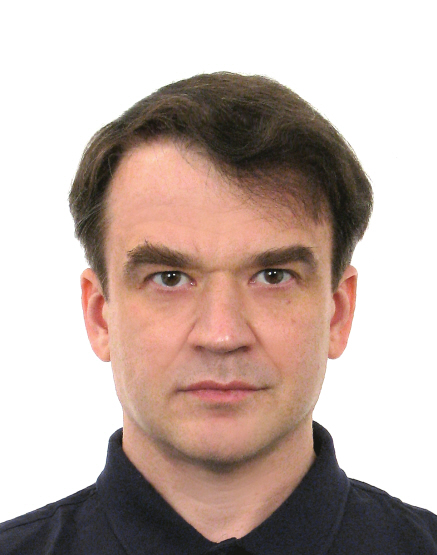
\includegraphics[width=0.8\columnwidth]{michurin.jpg}\\[\baselineskip] % Your photo
\footnotesize % \small % Smaller font size
Alexey Michurin \\ % Your name
\url{github.com/michurin} \\ % Your URL
\Sep
Gett, Yandex, VimpelCom, MSU \\
\Sep % Some whitespace
%\textbf{Backend} \\
Golang \\
Python \\
NodeJS \\
MapReduce/SQL/NoSQL \\
Linux \\
\Sep % Some whitespace
Billing \\
Inventory \\
Fraud prevention \\
ML infrastructure \\
\Sep % Some whitespace
%\textbf{Contacts} \\
\url{a.michurin@gmail.com} \\ % Your email address
+7 (906) 722-5401 \\ % Your phone number
\Sep % Some whitespace
%\textbf{Location} \\
Moscow, Russia \\ % Address 1
\vfill % Whitespace under this block to push it up under the photo
\end{flushright}
}

%----------------------------------------------------------------------------------------

%\makeatletter
%\let\oldsection\section%
%\renewcommand{\section}[1]{\leavevmode\unskip\vspace*{-\baselineskip}\oldsection{#1}}%
%\makeatother

\begin{document}

\userinformation % Print your information in the left column

\framebreak % End of the first column

%----------------------------------------------------------------------------------------
%	HEADING
%----------------------------------------------------------------------------------------

\cvheading{Alexey Michurin} % Large heading - your name

\cvsubheading{Backend Developer} % Subheading - your occupation/specialization

%----------------------------------------------------------------------------------------
%	ABOUT ME
%----------------------------------------------------------------------------------------

\aboutme{About Me}{I've been lucky to work on a bunch of amazing projects and learn from smartest people.
I believe my expertise might come in handy and you have challenging job.}

%----------------------------------------------------------------------------------------
%	EXPERIENCE
%----------------------------------------------------------------------------------------
\Sep % Extra whitespace after the end of a major section

\CVSection{Experience}

%------------------------------------------------

\CVItem{May 2018 -- present, Gett, Payments and Fraud prevention}{
Golang, Python, RabbitMQ, Postgres, PrestoDB, Redis, AWS.

The primary responsibility of our team is to support and develop payments infrastructure.
It made up of lots of internal and external integrations as well as parts of business logic.
I am also support existing fraud prevention system based on ML.
}

\CVItem{Jun 2016 -- May 2018, Yandex, Weather forecasting system}{
Python, MapReduce, MongoDB, distributed computing.

We developed distributed system, that fetched weather data from different sources
and produced weather forecast based on ML. I was engaged into process of
almost completely redevelopment of system. We got global and began to process
more data sources. I was mostly responsible for applying ML models and collecting
logs for training process. I designed not only the system itself, but also
degradation strategy, monitorings and other useful things.
}

\CVItem{Nov 2014 -- Jun 2016, Yandex, Advertising system}{
Python, Perl, MySQL, MapReduce, distributed computing.

Our team was focused on auction and bidding. I took part in development and investigations.
I also actively participated in design and development of RTB system.
I was feature owner and key developer for new banner enrichment feature.
In addition I contributed a bit to MapReduce engine.}

\vspace*{-6mm}  %%%%%%%%%% WHY!!!???

\CVItem{Dec 2006 -- Nov 2014, Vimpelcom (Beeline), Billing and Inventory}{
Python, Perl, MySQL, widespread distributed systems.

We managed Beeline WiFi and broadband networks with tens of thousands of network hardware
spread out over ten time zones. I was focused on control and monitoring system in
conjunction with billing system. For example, it switches shapers to align traffic to tariff and billing status of customer.
}

\Sep % Extra whitespace after the end of a major section

\CVSection{Education}

\CVItem{1992 -- 1998, Moscow State University}{Physical department. Master Of Science (Solid State Physics)}

\Sep % Extra whitespace after the end of a major section

\CVSection{(Fun) facts}

I worked in Moscow State University for 8 years after graduating.
I taught students, conducted researches, made speeches at conferences, wrote papers.
I worked abroad in international labs in Poland
(Warsaw University of Technology and International Laboratory of High Magnetic Fields and Low Temperatures, Wroclaw)
and Spain (University of Zaragoza).

%------------------------------------------------

%\Sep % Extra whitespace after the end of a major section

\clearpage

\end{document}
